\documentclass[11pt]{article}
\usepackage{amsmath}
\usepackage{amssymb}
\usepackage{graphicx}
\usepackage{fancyhdr}
\usepackage{enumerate}
%\usepackage{titlesec}
\usepackage[colorlinks=true,urlcolor=blue]{hyperref}
\usepackage{listings}
\usepackage{xcolor}
\definecolor{dkgreen}{rgb}{0,0.6,0}
%\usepackage{esvect}

%\titlespacing{\subsubsection}{0pt}{0pt}{0pt}
\lstset{language=python,
	frame=tb,
	numbers=none,
    basicstyle=\small\ttfamily,
    stringstyle=\color{dkgreen},
    %otherkeywords={0,1,2,3,4,5,6,7,8,9},
    morekeywords={TRUE,FALSE, def},
    deletekeywords={data,frame,length,as,character,plot,which,min,factor,mean,control},
    keywordstyle=\color{blue},
    commentstyle=\color{dkgreen},
}

% No page numbers
%\pagenumbering{gobble}



% MARGINS (DO NOT EDIT) ---------------------------------------------
\oddsidemargin  0.25in \evensidemargin 0.25in \topmargin -0.5in
\headheight 0in \headsep 0.1in
\textwidth  6.5in \textheight 9in
\parskip 1.25ex  \parindent 0ex \footskip 20pt
% ---------------------------------------------------------------------------------

% HEADER (DO NOT EDIT) -----------------------------------------------
\newcommand{\problemnumber}{0}
\newcommand{\myname}{name}
\newfont{\myfont}{cmssbx10 scaled 1000}
\pagestyle{fancy}
\fancyhead{}
\fancyhead[L]{\myfont Question \problemnumber, Assignment 2, CME 241 - Pablo Veyrat, pveyrat@stanford.edu}
%\fancyhead[R]{\bssnine \myname}
\newcommand{\newquestion}[1]{
\clearpage % page break and flush floats
\renewcommand{\problemnumber}{#1} % set problem number for header
\phantom{}  % Put something on the page so it shows
}
% ---------------------------------------------------------------------------------


% BEGIN HOMEWORK HERE
\begin{document}

% Problem 1.a
\newquestion{1}

You will find the code for this question in the \texttt{RL-book/Assignment2/assignment2\_code.py} file.

We created a class to define the state. This class which we called $\texttt{StateSnakeAndLadder}$ only has one attribute: it is the position on the grid. If the grid size is $100$ the State Space is $\{1,2,3,...,100\}$.

The structure of the transition probabilities can be found in the function \texttt{get\_transition\_map} of the $\texttt{StateSnakeAndLadderGame}$ class. 

\newquestion{2}
The graph of the probability distribution of time steps to finish the game is can be found here:

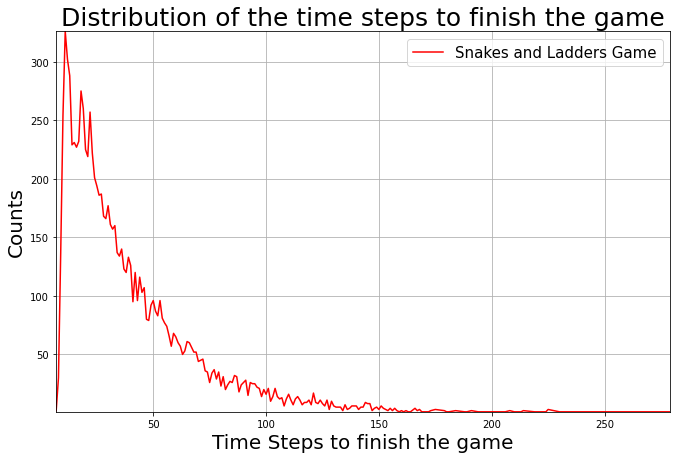
\includegraphics[scale=0.75]{/Users/pabloveyrat/Documents/Stanford/Winter21/CME241/Assignments/RL-book/Assignment2/Distribution_Timesteps.png}

We used the code in the \texttt{RL-book/Assignment2/assignment2\_code.py} file to generate it.

\newquestion{3}
Let us solve the Frog Puzzle. We want to find out the expected number of steps required when there are $n$ leaves ahead.

Let $K_n$ be this number.

We first have that $K_0 = 0$.

Let us name the leaves. We will choose here to number them according to their distance from the destination, i.e. the last leaf (the one at which we stop counting) is going to be leaf 0, and the leaf we start at is leaf $n$.

Note that in this case, Markov property is respected: when the frog is on a given leaf, the expected number of jumps remaining only depends on the leaf on which the frog is and not on the leaves where the frog was before that leaf.

Hence, after the first leaf, if the frog lands on leaf $i$, with $i\in \{0, ..., n-1\}$, the expected value of the remaining steps will be $K_i$.

Besides this Markov Assumption, with the law of total probability, we get:
\[K_n = 1+ \frac{1}{n}\sum_{i=0}^{n-1} K_i =  \frac{1}{n}\sum_{i=0}^{n-1}\frac{1}{n}(1+ K_i)\]
This can be rewritten:
\[n(K_n -1)= \sum_{i=0}^{n-1} K_i\]
Similarly, we get that, as $n$ has been chosen generically (for $n\geq1$):
\[(n-1)(K_{n-1} -1)= \sum_{i=0}^{n-2} K_i\]
We can thus take advantage of the fact that the differences between the two sums above will simplify. We get:
\[n(K_n -1) - (n-1)(K_{n-1} -1) = K_{n-1} \]
Hence:
\[nK_n -n -(n-1)K_{n-1} + (n-1) = K_{n-1}\]
\[K_n = K_{n-1} + \frac{1}{n}\]
By using the fact that $K_0 = 0$ and that $\sum_{i=1}^{n} (K_i - K_{i-1}) = K_n - K_0$, we get that:
\[K_n = \sum_{i=1}^n \frac{1}{i}\]

\newquestion{4}
The Bellman equation gives us that the value function is such that:
\[V(s) = R(s) + \gamma \sum_{s^{'} \in \texttt{N}} P(s,s^{'}) V(s^{'}) \]

And the expectation of the number of dice rolls to finish the game is:
\[\mathbb{E}(N_{steps}|state = s) = 1 + \sum_{i=1}^{\text{grid\_size}} P(s,i) \mathbb{E}(N_{steps}|state = i)\] 

Hence, if we let $R(s) = 1$ for any non-terminating state, and choose to have $\gamma = 1$, then we can determine the expected number of dice rolls to finish the game just by using the \texttt{get\_value\_function\_vec} of the FiniteMarkovRewardProcess instance corresponding to the process.

This is what we did in the code.

\newquestion{5}
To compute the Value Function for any discount factor $0\leq \gamma \leq 1$, as:
\[V(s) = \mathbb{E}(R_{t+1}|S_t =s) + \gamma \mathbb{E}(R_{t+2}|S_t =s) + \gamma^2 \mathbb{E}(R_{t+3}|S_t =s) + ... \]
We can use simulations and simulate \texttt{num\_traces} reward traces for a given starting state and for each trace compute the discounted sum of rewards.

We then get an estimate of the value function by taking the mean of the discounted sum of rewards across the different traces we generated.

This is what we did in the code for this problem.

%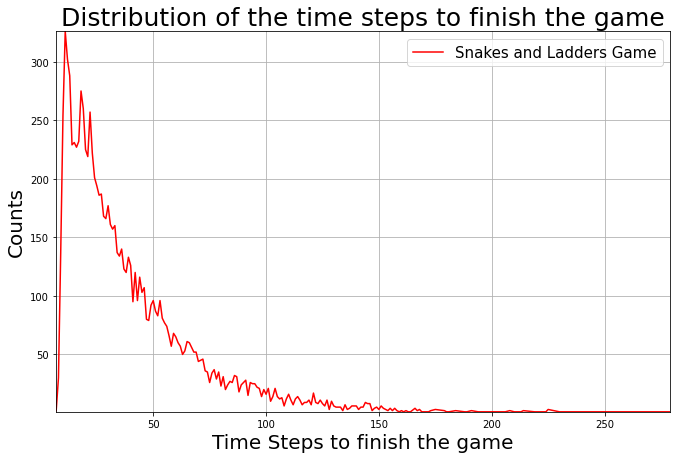
\includegraphics[scale=0.75]{/Users/pabloveyrat/Documents/Stanford/Winter21/CME241/Assignments/RL-book/Assignment2/Distribution_Timesteps.png}





\end{document}